\documentclass[tikz,border=4pt]{standalone}
\usepackage{amsmath}
\begin{document}
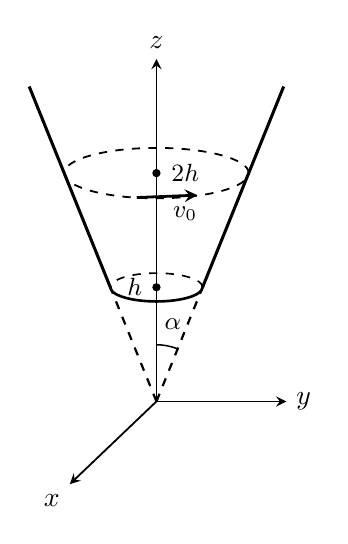
\begin{tikzpicture}[>=stealth, thick, scale=1.0]
  % 3D axes at apex O(0,0): z up, y right, x down-left
  \draw[->, line width=0.65pt] (0, 0) -- (0, 4.35) node[above] {$z$};
  \draw[->, line width=0.65pt] (0, 0) -- (1.65, 0) node[right] {$y$};
  \draw[->, line width=0.65pt] (0, 0) -- (-1.1, -1.05) node[below left] {$x$};

  % Cone half-angle alpha = 22 deg (tan(22) = 0.4040)
  % Truncation height h -> z_h = 1.45, initial height 2h -> z_2h = 2.90, top -> z_top = 4.0
  \def\tana{0.404}
  \def\zh{1.45}
  \def\zhh{2.90}
  \def\ztop{4.0}
  \pgfmathsetmacro{\rh}{\zh*\tana}
  \pgfmathsetmacro{\rhh}{\zhh*\tana}
  \pgfmathsetmacro{\rtop}{\ztop*\tana}

  % Dashed cone extensions from apex to z = h
  \draw[dashed, line width=0.8pt] (0, 0) -- (-\rh, \zh);
  \draw[dashed, line width=0.8pt] (0, 0) -- (\rh, \zh);

  % Solid cone walls from z = h to z = z_top
  \draw[line width=1.1pt] (-\rh, \zh) -- (-\rtop, \ztop);
  \draw[line width=1.1pt] (\rh, \zh) -- (\rtop, \ztop);

  % Bottom opening ellipse at z = h (front solid, back dashed)
  \draw[line width=0.95pt] (-\rh, \zh) arc[start angle=180, end angle=360, x radius=\rh, y radius=0.18];
  \draw[dashed, line width=0.6pt] (\rh, \zh) arc[start angle=0, end angle=180, x radius=\rh, y radius=0.18];

  % Circle at z = 2h (dashed)
  \draw[dashed, line width=0.65pt] (0, \zhh) ellipse[x radius=\rhh, y radius=0.32];

  % Height markers h and 2h on z-axis
  \fill (0, \zh) circle (1.5pt);
  \node[left, font=\small] at (-0.05, \zh) {$h$};
  \fill (0, \zhh) circle (1.5pt);
  \node[right, font=\small] at (0.06, \zhh) {$2h$};

  % Initial velocity arrow v0 at front of z = 2h circle
  \draw[->, line width=1.0pt] (-0.25, \zhh - 0.31) -- (0.52, \zhh - 0.28);
  \node[below right, font=\small] at (0.08, \zhh - 0.30) {$v_0$};

  % Angle alpha between z-axis and right dashed generator
  \draw[line width=0.55pt] (0, 0.72) arc[start angle=90, end angle=68, radius=0.72];
  \node[font=\small] at (78:1.0) {$\alpha$};
\end{tikzpicture}
\end{document}
